%------------------------------------------------
% main.tex - MA1500 2015-16
%------------------------------------------------
\documentclass{camel}

% options
% \cymraegtrue
% \screentrue
% \booklettrue
% \blankstrue
% \answerstrue

% mandatory settings
\academicyear{2015-16}
\modulecode{MA1234}
\moduletitle{Probability Theory}
\booknumber{1}

% optional settings
\booktitle{Lecture Notes}
%\bookauthor{Dafydd Evans}
%\bookdate{\today}
\bookversion{v1.0}

% figures
\usepackage{graphicx}
\graphicspath{{./figures/}}
\DeclareGraphicsExtensions{.png,.pdf,.jpeg,.gif}
\usepackage{caption}
\usepackage{subcaption}
%\captionsetup[subfigure]{labelformat=empty}
%\captionsetup[figure]{skip=2ex}

% naughty
\def\it{\item}
\def\bit{\begin{itemize}}
\def\eit{\end{itemize}} 
\def\ben{\begin{enumerate}}
\def\een{\end{enumerate}}

% macros
\newcommand{\Z}{\mathbb{Z}}
\newcommand{\N}{\mathbb{N}}
\newcommand{\R}{\mathbb{R}}
\newcommand{\C}{\mathbb{C}}
\newcommand{\supp}{\text{supp}}
\newcommand{\prob}{\mathbb{P}}
\newcommand{\expe}{\mathbb{E}}
\newcommand{\var}{\text{Var}}
\newcommand{\cov}{\text{Cov}}
\newcommand{\mode}{\text{Mode}}


%------------------------------------------------
\begin{document}
\makefrontmatter
%------------------------------------------------
% !TEX root = main.tex
%======================================================================
\chapter{Set Theory}\label{chap:sets}
%======================================================================

%----------------------------------------------------------------------
\section{Elementary set theory}
%----------------------------------------------------------------------

A set is a collection of distinct \emph{elements}.
\bit
\it If $a$ is an element of the set $A$, we denote this by $a\in A$.
\it If $a$ is \emph{not} an element of $A$, we denote this by $a\notin A$.
\it The \emph{cardinality} of a set is the number of elements it contains.
\it The \emph{empty set} contains no elements, and is denoted by $\emptyset$.
\eit

Algebra is the study of \emph{operations} and \emph{relations}.
\bit
\it The basic relations of set algebra are \emph{set inclusion} and \emph{set equality}.
\it The basic operations of set algebra are \emph{complementation}, \emph{union} and \emph{intersection}.
\eit

%----------------------------------------------------------------------
\break
\subsection{Set relations}
%----------------------------------------------------------------------

% definition: set inclusion, set equality
\begin{definition}
Let $A$ and $B$ be sets. 
\ben
\it If every element of $A$ is also an element of $B$, we say that $A$ is a \emph{subset} of $B$.
\par This is denoted by $A\subseteq B$.
\it If every element of $A$ is an element of $B$, and every element of $B$ is an element of $A$, we say that $A$ and $B$ are \emph{equal}. 
\par This is denoted by $A=B$.
\it If $A$ is a subset of $B$, but $A$ is not equal to $B$, we say that $A$ is a \emph{proper subset} of $B$. 
\par This is denoted by $A\subset B$.
\een
\end{definition}

% picture: set inclusion
%\picbox{5cm}

% example
\begin{example}
Let $A=\{a,b\}$, $B=\{a,b\}$ and $C=\{a,b,c\}$.
\bit
\it $A$ is a subset of $B$: $A\subseteq B$,
\it $A$ is also equal to $B$: $A=B$, and
\it $A$ is a proper subset of $C$: $A\subset C$.
\eit
\end{example}

%----------------------------------------------------------------------
\break
\subsection{Set operations}
%----------------------------------------------------------------------
\begin{definition}
Let $A$, $B$ and $\Omega$ be sets, with $A,B\subseteq \Omega$.
\ben
\it The \emph{union} of $A$ and $B$ is the set
$$
A\cup B = \{a\in \Omega: a\in A \text{ or }a\in B\}.
$$
\it The \emph{intersection} of $A$ and $B$ is the set
$$
A\cap B = \{a\in \Omega: a\in A \text{ and }a\in B\}.
$$
\it The \emph{complement} of $A$ is the set 
$$
A^c=\{a\in \Omega:a\notin A\}.
$$
\een
\end{definition}

% example
\begin{example}
Let $A=\{a,b\}$, $B=\{b,c\}$ and $\Omega=\{a,b,c,d\}$.
\par
Then
$A\cup B = \{a,b,c\}$, $A\cap B = \{b\}$ and $A^c = \{c,d\}$.
\end{example}

\break % <<

% figure: basic set operations
\begin{figure}[htb]
\centering
\begin{tabular}{ccc}
	\begin{subfigure}{.25\textwidth}
	\resizebox{\linewidth}{!}{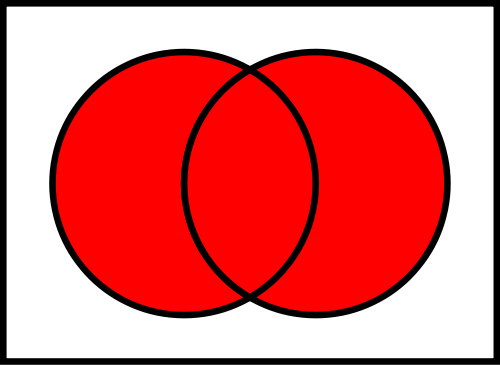
\includegraphics{AcupB}}
	\caption{Union}
	\end{subfigure}
&
	\begin{subfigure}{.25\textwidth}
	\resizebox{\linewidth}{!}{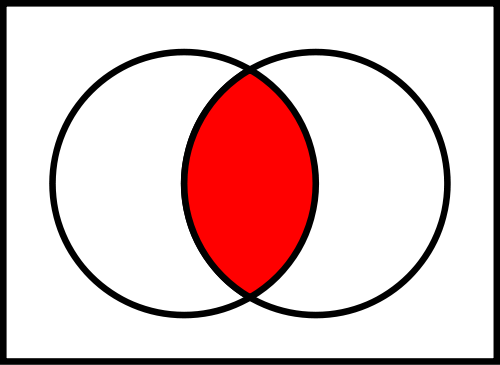
\includegraphics{AcapB}}
	\caption{Intersection}
	\end{subfigure}
&
	\begin{subfigure}{.25\textwidth}
	\resizebox{\linewidth}{!}{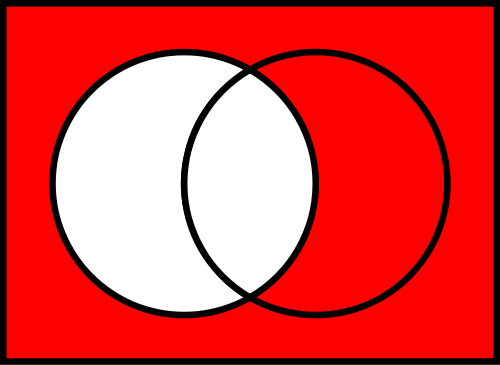
\includegraphics{Acomp}}
	\caption{Complement}
	\end{subfigure}
\end{tabular}
\end{figure}

\begin{center}
\begin{tabular}{|c|c||c|c|c|} \hline
Set Theory 		& 			& Logic			&		& \\ \hline
Union			& $A\cup B$	& Disjunction 	& OR 	& $\lor$	\\
Intersection		& $A\cap B$	& Conjunction	& AND 	& $\land$\\
Complement		& $A^c$		& Negation		& NOT 	& $\lnot$	\\ \hline
\end{tabular}
\end{center}

\break % <<

%----------------------------------------------------------------------
\subsection{Set algebra}
%----------------------------------------------------------------------
\begin{definition}
\ben
\it Commutative property.
\bit 
\it $A\cup B = B\cup A$,
\it $A\cap B = B\cap A$.
\eit
\it Associative property.
\bit 
\it $(A\cup B)\cup C = A\cup (B\cup C)$,
\it $(A\cap B)\cap C = A\cap (B\cap C)$.
\eit
\it Distributive property.
\bit 
\it $A\cup (B\cap C) = (A\cup B)\cap(A\cup C)$,
\it $A\cap (B\cup C) = (A\cap B)\cup(A\cap C)$.
\eit
\een
\end{definition}

\begin{remark}
A statement such as $A\cup B\cap C$ is ambiguous. 
\end{remark}

%----------------------------------------------------------------------
\section{De Morgan's laws}
%----------------------------------------------------------------------
Union and intersection swap roles under complementation.

\begin{theorem}\label{thm:demorgan_simple}
\ben
\it $(A\cup B)^c = A^c\cap B^c$.
\it $(A\cap B)^c = A^c\cup B^c$.
\een
\end{theorem}

\begin{proof}
\begin{enumerate}
\item % part (1)
Let $a\in(A\cup B)^c$. Then $a\notin A$ and $a\notin B$, so $a\in A^c\cap B^c$.
Hence $(A\cup B)^c\subseteq A^c\cap B^c$.\par
Let $a\in A^c\cap B^c$. Then $a\notin A$ and $a\notin B$, so $a\notin A\cup B$.
Hence $A^c\cap B^c\subseteq (A\cup B)^c$.\par
Thus it follows that $(A\cup B)^c = A^c\cap B^c$.
\item % part (2)
Apply part (1) to the sets $A^c$ and $B^c$: $(A^c\cup B^c)^c = A\cap B$.\par
Then take the complement of both sides: $(A\cap B)^c = A^c\cup B^c$.
\end{enumerate}
\end{proof}

%----------------------------------------------------------------------
\section{Set difference}
%----------------------------------------------------------------------
\begin{definition}
Let $A$, $B$ and $\Omega$ be sets, with $A,B\subseteq \Omega$.
\ben
\it The \emph{set difference} between $A$ and $B$ is the set
$$
A\setminus B = \{a\in \Omega : a\in A \text{ and } a\notin B\}. % = A\cap B^c.
$$
\it The \emph{symmetric difference} between $A$ and $B$ is the set 
$$
A\bigtriangleup B = (A\setminus B) \cup (B\setminus A). %= (A\cap B^c)\cup (B\cap A^c). 
$$
\een
\end{definition}

\bit
\it $A\setminus B$ is the set of points that are in $A$ but not in $B$.
\it $A\bigtriangleup B$ is the set of points that are in either $A$ or $B$, but not both.
\eit

% example
\begin{example}
Let $A=\{a,b\}$ and $B=\{b,c\}$. Then
\bit
\it $A\setminus B = \{a\}$
\it $A\bigtriangleup B = \{a,c\}$.
\eit
\end{example}

\break % <<


%----------------------------------------------------------------------
%\section*{Appendix: Set operations}
%----------------------------------------------------------------------
% figure
\begin{figure}[htb]
\centering

\begin{tabular}{cccc}	
\begin{subfigure}{.15\textwidth}
\resizebox{\linewidth}{!}{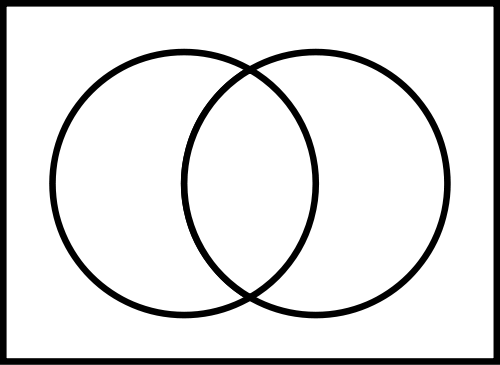
\includegraphics{emptyset}}
\caption{$\emptyset$}
\end{subfigure}
&
\begin{subfigure}{.15\textwidth}
\resizebox{\linewidth}{!}{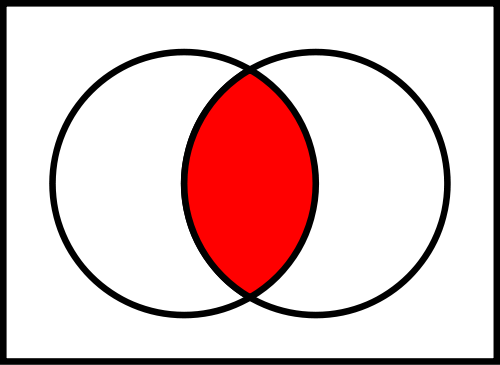
\includegraphics{AcapB}}
\caption{$A\cap B$}
\end{subfigure}
&
\begin{subfigure}{.15\textwidth}
\resizebox{\linewidth}{!}{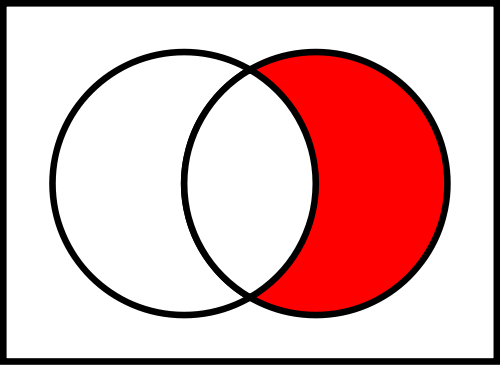
\includegraphics{BminusA}}
\caption{$B\setminus A$}
\end{subfigure}
&
\begin{subfigure}{.15\textwidth}
\resizebox{\linewidth}{!}{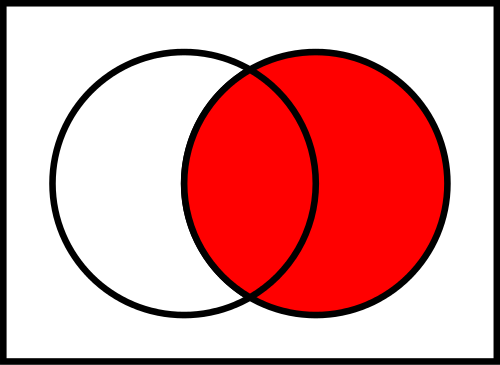
\includegraphics{setB}}
\caption{$B$}
\end{subfigure}
\end{tabular}

\begin{tabular}{cccc}
\begin{subfigure}{.15\textwidth}
\resizebox{\linewidth}{!}{
\includegraphics{AcupB_comp}}
\caption{$(A\cup B)^c$}
\end{subfigure}
&
\begin{subfigure}{.15\textwidth}
\resizebox{\linewidth}{!}{
\includegraphics{symdiff_comp}}
\caption{$(A\bigtriangleup B)^c$}
\end{subfigure}
&
\begin{subfigure}{.15\textwidth}
\resizebox{\linewidth}{!}{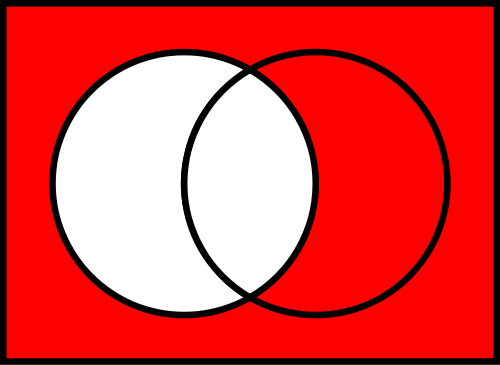
\includegraphics{Acomp}}
\caption{$A^c$}
\end{subfigure}
&
\begin{subfigure}{.15\textwidth}
\resizebox{\linewidth}{!}{
\includegraphics{AminusB_comp}}
\caption{$(A\setminus B)^c$}
\end{subfigure}
\end{tabular}

\begin{tabular}{cccc}
\begin{subfigure}{.15\textwidth}
\resizebox{\linewidth}{!}{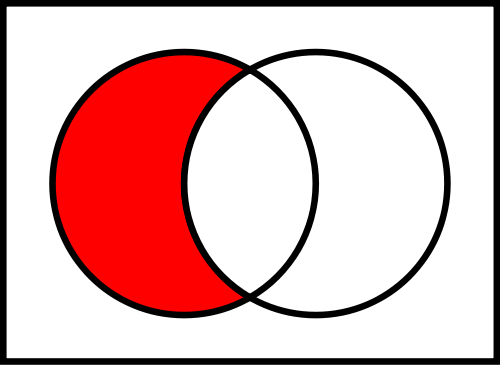
\includegraphics{AminusB}}
\caption{$A\setminus B$}
\end{subfigure}
&
\begin{subfigure}{.15\textwidth}
\resizebox{\linewidth}{!}{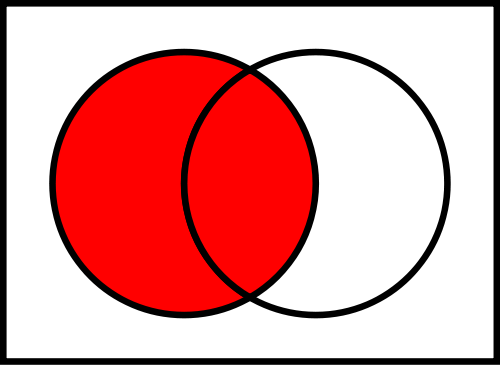
\includegraphics{setA}}
\caption{$A$}
\end{subfigure}
&
\begin{subfigure}{.15\textwidth}
\resizebox{\linewidth}{!}{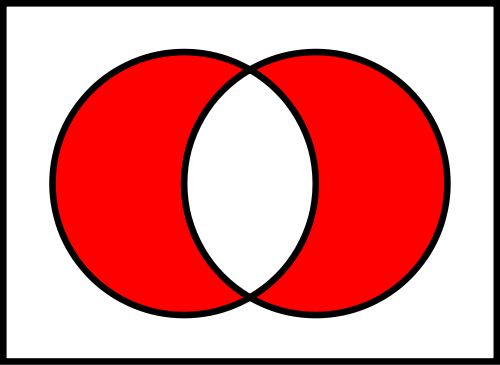
\includegraphics{symdiff}}
\caption{$A\bigtriangleup B$}
\end{subfigure}
&
\begin{subfigure}{.15\textwidth}
\resizebox{\linewidth}{!}{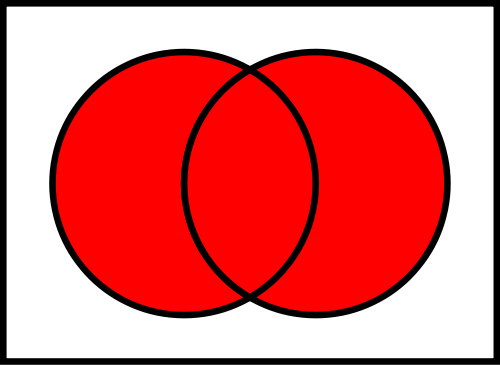
\includegraphics{AcupB}}
\caption{$A\cup B$}
\end{subfigure}
\end{tabular}

\begin{tabular}{cccc}
\begin{subfigure}{.15\textwidth}
\resizebox{\linewidth}{!}{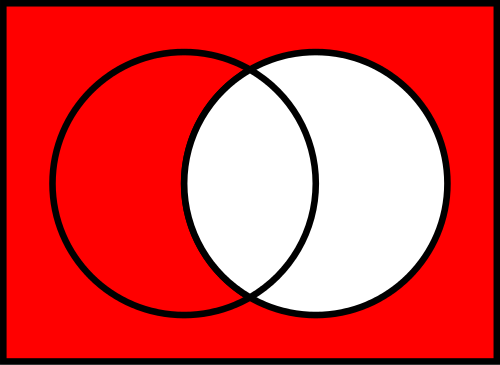
\includegraphics{Bcomp}}
\caption{$B^c$}
\end{subfigure}
&
\begin{subfigure}{.15\textwidth}
\resizebox{\linewidth}{!}{
\includegraphics{BminusA_comp}}
\caption{$(B\setminus A)^c$}
\end{subfigure}
&
\begin{subfigure}{.15\textwidth}
\resizebox{\linewidth}{!}{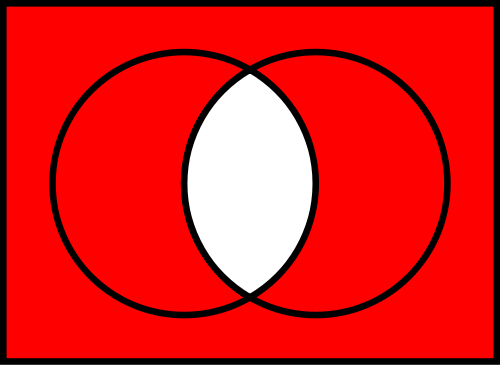
\includegraphics{AcapB_comp}}
\caption{$(A\cap B)^c$}
\end{subfigure}
&
\begin{subfigure}{.15\textwidth}
\resizebox{\linewidth}{!}{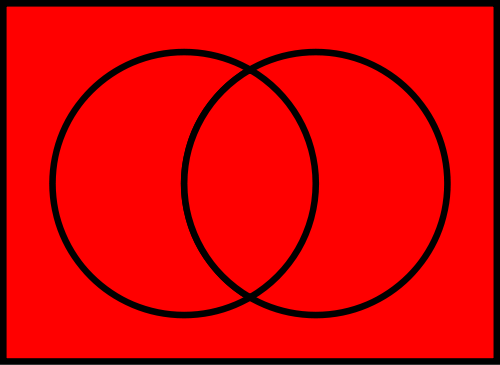
\includegraphics{universe}}
\caption{$\emptyset^c$}
\end{subfigure}
\end{tabular}
\caption{Set Operations ($A$ on the left, $B$ on the right).\label{fig:set-operations}}
\end{figure}

%----------------------------------------------------------------------
\section{Exercises}
% !TEX root = main.tex

\begin{exercise}
\begin{questions}
\question
Illustrate the basic set operations using Venn diagrams.%, as shown in Figure~\ref{fig:set-operations}.
\question
State and prove De Morgan's laws.
\end{questions}
\end{exercise}

%======================================================================
\endinput
%======================================================================

%----------------------------------------------------------------------
%======================================================================
\endinput
%======================================================================

% !TEX root = main.tex
%======================================================================
\chapter{Events}\label{chap:events}
%======================================================================

\section*{A brief history of probability}
Games of chance have been played since antiquity, but the mathematical principles of chance and uncertainty were first established only in the 17th century.

\vspace*{4ex}
\begin{tabular}{lll}
1654		& Classical principles 	& Blaise Pascal (1623--1662) \\
    		&						& Pierre de Fermat (1601--1665)  \\
1657		& \textit{De Ratiociniis in Ludo Aleae} & Christiaan Huygens (1629--1695) \\
1713		& \textit{Ars Conjectandi} & Jakob Bernoulli (1654--1705) \\ 
1718		& \textit{The Doctrine of Chances} & Abraham de Moivre (1667--1754) \\
1812		& \textit{Theorie Analytique des Probabilites} & Pierre de Laplace (1749-1827) \\
1919		& Relative frequency & Richard von Mises (1883--1953) \\
1933		& Modern axiomatic theory & Andrey Kolmogorov (1903--1987)\\
\end{tabular}

%----------------------------------------------------------------------
\section{Sample spaces}
%----------------------------------------------------------------------
% defn: random_experiment/outcome/sample_space
\begin{definition}
\ben
\it
Any process of observation or measurement will be called an \emph{experiment} or \emph{trial}.
\it
Any experiment whose outcome is uncertain is called a \emph{random experiment}.
\it
A random experiment has a set of possible \emph{outcomes}.
\it
Each time a random experiment is performed, \emph{exactly one} of its outcomes will occur.
\it
The set of all possible outcomes is called the \emph{sample space} of the experiment, denoted by $\Omega$.
\it
Outcomes are also called \emph{elementary events}, and denoted by $\omega\in\Omega$.
\een
\end{definition}

\break

% example: sample spaces
\begin{example}
For any random experiment, the sample space is the set of all possible outcomes:
\begin{tabbing}
\underline{Experiment}\hspace{50ex} \= \underline{Sample space} \\[1ex]
A coin is tossed once.	\> $\Omega = \{H,T\}$ \\
A six-sided die is rolled once.	\> $\Omega=\{1,2,3,4,5,6\}$ \\
A coin is tossed repeatedly until a head occurs. \> $\Omega = \{1,2,3,\ldots\}$ \\
The height of a randomly chosen student is measured: \> $\Omega = [0,\infty)$
\end{tabbing}
\end{example}

%----------------------------------------------------------------------
\section{Events}
%----------------------------------------------------------------------

% defn: events
\begin{definition}
\bit
\it An \emph{event} $A$ is a subset of the sample space, $\Omega$. 
\it If outcome $\omega$ occurs, we say that event $A$ \emph{occurs} if and only if $\omega\in A$.
\it Two events $A$ and $B$ with $A\cap B=\emptyset$ are called \emph{disjoint} or \emph{mutually exclusive}.
\it The empty set $\emptyset$ is called the \emph{impossible event}.
\it The sample space $\Omega$ is called the \emph{certain event}.
\eit
\end{definition}

\begin{remark}
\bit
\it If $A$ occurs and $A\subseteq B$, then $B$ must also occur.
\it If $A$ occurs and $A\cap B=\emptyset$, then $B$ does not occur. 
\eit
\end{remark}

\break

% example: die
\begin{example}
A die is rolled once. The sample space can be represented by $\Omega=\{1,2,3,4,5,6\}$.\par
We may be interested in whether or not the following events occur:
\begin{tabbing}
\underline{Event}\qquad\qquad\qquad\qquad\qquad\qquad\qquad\qquad\qquad\qquad\qquad\qquad\=\underline{Subset} \\ 
The outcome is the number $1$.	\> $A = \{1\}$ \\
The outcome is an even number.	\> $A = \{2,4,6\}$ \\
The outcome is even but does not exceed $3$.	\> $A = \{2,4,6\}\cap\{1,2,3\}$ \\
The outcome is not even			\> $A = \Omega\setminus\{2,4,6\}$
\end{tabbing}
\end{example}

%----------------------------------------------------------------------
\section{Families of events}
%----------------------------------------------------------------------
\begin{definition}
Let $\Omega$ be any set. 
\ben
\it The set of all subsets of $\Omega$ is called its \emph{power set}, which we denote by $\mathcal{P}(\Omega)$.
\it Any subset of $\mathcal{P}(\Omega)$ is called a \emph{family of sets over $\Omega$}.
\een
\end{definition}

Let $\Omega$ be the sample space of some random experiment. 
If we are interested in events $A$ and $B$, we must also be interested in whether:

\begin{itemize}
\item event $A$ occurs \emph{or} event $B$ occurs -- this is the event $A\cup B$,
\item event $A$ occurs \emph{and} event $B$ occurs -- this is the event $A\cap B$,
\item event $A$ does \emph{not} occur -- this is the event $A^c$.
\end{itemize}

\smallskip
We cannot therefore use arbitrary families of sets over $\Omega$ as the basis for investigating random experiments. Instead, we allow only families that are \emph{closed} under certain set operations.

\break

\begin{definition}
A family of sets $\mathcal{F}$ over $\Omega$ is said to be
\ben
\it \emph{closed under complementation} if $A^c\in\mathcal{F}$ for every $A\in\mathcal{F}$, 
\it \emph{closed under pairwise unions} if $A\cup B\in\mathcal{F}$ for every $A,B\in\mathcal{F}$, 
\it \emph{closed under finite unions}	if $\bigcup_{i=1}^{n} A_i\in\mathcal{F}$ for every $A_1,A_2,\ldots A_n\in\mathcal{F}$,
\een
\end{definition}

% defn: fields of sets
\begin{definition}
A family of sets $\mathcal{F}$ over $\Omega$ is called a \emph{field of sets} over $\Omega$ if
\begin{enumerate}
\item $\Omega\in\mathcal{F}$,
\item $\mathcal{F}$ is closed under complementation, and
\item $\mathcal{F}$ is closed under pairwise unions.
\end{enumerate}
\end{definition}

\break

% example
\begin{example}\label{ex:fields_of_sets}
A six-sided die is rolled once, and the score is observed. A suitable sample space for this experiment is the set 
$\Omega=\{1,2,3,4,5,6\}$. The power set of $\Omega$ will always provide a field of sets to work with. However, suppose we are only interested in whether or not the outcome is an even number. In this case, we need only consider the following family of events:
\[
\mathcal{F} = \big\{\emptyset, \{1,3,5\}, \{2,4,6\}, \{1,2,3,4,5,6\}\big\}.
\]
We can see that $\mathcal{F}$ is a field of sets over $\Omega$, because
\ben
\it it contains the sample space $\{1,2,3,4,5,6\}$,
\it the complement of every set in $\mathcal{F}$ is also contained in $\mathcal{F}$, and
\it the union of any two sets in $\mathcal{F}$ is also contained in $\mathcal{F}$.
\een
\end{example}

\break

% properties of fields
\begin{theorem}[Properties of fields]
Let $\mathcal{F}$ be a field over $\Omega$. Then
\begin{enumerate}
\item $\emptyset\in\mathcal{F}$,
\item $\mathcal{F}$ is closed under pairwise intersections,
\item $\mathcal{F}$ is closed under set differences.
\end{enumerate}
\end{theorem}

\begin{proof}
\begin{enumerate}
\item
We know that $\emptyset = \Omega^c$, and that $\Omega\in\mathcal{F}$. Because $\mathcal{F}$ is closed under complementation, it thus follows that $\emptyset\in\mathcal{F}$.
\item
Let $A,B\in\mathcal{F}$. By De Morgan's laws, we have that $A\cap B = (A^c\cup B^c)^c$. Because $\mathcal{F}$ is closed under complementation and pairwise unions, it thus follows that $A\cap B\in\mathcal{F}$.
\item
Let $A,B\in\mathcal{F}$. Set difference can be written as $A\setminus B = A\cap B^c$. Furthermore, by De Morgan's laws we see that $A\cap B^c = (A^c\cup B)^c$. Because $\mathcal{F}$ is closed under complementation and pairwise unions, it thus follows that $A\setminus B\in\mathcal{F}$.
\end{enumerate}
\end{proof}

%----------------------------------------------------------------------
\section{Terminology}
%----------------------------------------------------------------------
\begin{table}[h]
\centering\small
\begin{tabular}{|c|l|l|} \hline
Notation 			& Set theory			& Probability theory \\ \hline
$\Omega$			& Universal set			& Sample space \\ 
$\omega\in\Omega$	& Element of $\Omega$	& Elementary event, outcome \\
$A\subseteq\Omega$	& Subset of $\Omega$	& Event $A$ \\
$A\subseteq B$		& Inclusion				& If $A$ occurs, then $B$ occurs \\
$A\cup B$			& Union					& $A$ or $B$ occurs \\ 
$A\cap B$			& Intersection			& $A$ and $B$ occur\\ 
$A^c$				& Complement of $A$		& $A$ does not occur \\
$A\setminus B$		& Difference			& $A$ occurs, but $B$ does not \\
$A\bigtriangleup B$	& Symmetric difference	& $A$ or $B$ occurs, but not both \\
$\emptyset$			& Empty set 			& Impossible event \\
$\Omega$			& Universal set			& Certain event \\ \hline
\end{tabular}
%\caption*{Table of correspondence (Grimmett \& Stirzaker 2001).}
\end{table}


%----------------------------------------------------------------------
\section{Exercises}
% !TEX root = main.tex

\begin{exercise}
\begin{questions}
%----------------------------------------
% events
\question
Identify a sample space, and the subset corresponding to event $A$, in each of the following scenarios:
\begin{parts}
%--------------------
\part A coin is tossed three times. $A$ is the event that at least two heads are obtained.
\begin{answer}
\par
$\Omega	= \{HHH, HHT, HTH, THH, HTT, THT, TTH, TTT\}$ and $A = \{HHH, HHT, HTH, THH\}$. Alternatively, if we are only interested in the number of heads, we could take $\Omega=\{0,1,2,3\}$ and $A=\{2,3\}$.
\end{answer}
%--------------------
\part A game of football is played. $A$ is the event that the match ends in a draw.
\begin{answer}
$\Omega=\{(a,b):a,b = 0,1,2,\ldots\}$ and $A=\{(a,b): a=b\}$ where $a$ and $b$ are the numbers of goals scored by the first and second teams, respectively. Note that this is a (countably) infinite set. 
\par
Alternatively, we could take $\Omega=\{W,D,L\}$ and $A=\{D\}$ where $W,D,L$ are respectively the events that the first team wins, draws or loses the game.
\end{answer}
%--------------------
\part A couple have two children. $A$ is the event that both are girls.
\begin{answer}
$\Omega=\{GG,GB,BG,BB\}$ and $A=\{GG\}$.
\par
Alternatively, we could take $\Omega=\{0,1,2\}$ and $A=\{2\}$.
\end{answer}
%--------------------
\part A shot hits a circular target of radius 10cm. $A$ is the event that the shot hits within 3cm of the centre.
\begin{answer}
$\Omega=\{(x,y): x^2+y^2\leq 10^2\}$ and $A=\{(x,y): x^2+y^2\leq 3^2\}$.
\end{answer}
\end{parts}

%----------------------------------------
% properties of fields
\question
A family of sets $\mathcal{F}$ over $\Omega$ is said to be
\bit
\it \emph{closed under finite unions} if $A_1\cup A_2\cup\ldots\cup A_n\in\mathcal{F}$ whenever $A_1,A_2,\ldots A_n\in\mathcal{F}$,
\it \emph{closed under finite intersections} if $A_1\cap A_2\cap\ldots\cap A_n\in\mathcal{F}$ whenever $A_1,A_2,\ldots A_n\in\mathcal{F}$.
\eit
Suppose that $\mathcal{F}$ is a field of sets over $\Omega$. Show that
\begin{parts}
%--------------------
%--------------------
\part $\mathcal{F}$ is closed under finite unions, and that
\begin{answer}
Proof by induction. Suppose that $\mathcal{F}$ is closed under unions of $n$ sets (where $n\geq 2$). Let $A_1,A_2,\ldots,A_{n+1}\in\mathcal{F}$. By the inductive hypothesis, $\cup_{i=1}^nA_i\in\mathcal{F}$. Thus $\cup_{i=1}^{n+1} A_i = \big[\cup_{i=1}^{n} A_i\big] \cup A_{n+1} \in\mathcal{F}$, because $\mathcal{F}$ is closed under pairwise unions.
\end{answer}
%--------------------
\part $\mathcal{F}$ is closed under finite intersections.
\begin{answer}
Let $A_1,A_2,\ldots,A_n\in\mathcal{F}$. Then $\cap_{i=1}^n A_i = \big[\cup_{i=1}^n A_i^c\big]^c$ (De Morgan's laws). Hence $\cap_{i=1}^n A_i\in\mathcal{F}$ because $\mathcal{F}$ is closed under complementation and finite unions. 
\end{answer}
%--------------------
\end{parts}
%----------------------------------------
\end{questions}
\end{exercise}

%======================================================================
\endinput
%======================================================================

%----------------------------------------------------------------------

%======================================================================
\endinput
%======================================================================

% !TEX root = main.tex
%======================================================================
\chapter{Probability}\label{chap:prob}
%======================================================================

%----------------------------------------------------------------------
\section{Probability measures}
%----------------------------------------------------------------------
Probability is defined to be a \emph{function} that assigns numerical value to random events.

\begin{definition}
Let $\Omega$ be the sample space of some random experiment, and let $\mathcal{F}$ be a field of sets over $\Omega$. A \emph{probability measure} on $(\Omega,\mathcal{F})$ is a function 
\[
\begin{array}{rccl}
	\prob:	& \mathcal{F}	& \to	& [0,1] \\[1ex]
			& A				& \mapsto	& \prob(A)
\end{array}
\]
such that $\prob(\Omega) = 1$, and for any countable collection of pairwise disjoint events $\{A_1,A_2,\ldots\}$,
\[
\prob\left(\bigcup_{i=1}^\infty A_i\right) = \sum_{i=1}^{\infty} \prob(A_i).
\]
The triple $(\Omega,\mathcal{F},\prob)$ is called a \emph{probability space}.
\end{definition}

\begin{remark}
\bit
\it The second property is called \emph{countable additivity}.
\it The number $\prob(A)$ is called the \emph{probability} of event $A\in\mathcal{F}$.
\eit
\end{remark}

\break

% example: die
\begin{example}
Consider a random experiment in which a fair six-sided die is rolled once.
\bit
\it A suitable sample space for the experiment is $\Omega=\{1,2,3,4,5,6\}$.
\it A suitable field of events for the experiment is the power set, $\mathcal{F} = \mathcal{P}(\Omega)$.
\it Because the die is fair, a suitable probability measure is given by the function
\[\begin{array}{rcl}
\prob:	\mathcal{F} & \to 		& [0,1] \\
		A			& \mapsto 	& \frac{1}{6}|A|, \qquad\text{where $|A|$ denotes the cardinality of $A$.}

\end{array}\] 
\eit

\begin{tabbing}
\underline{Event}\qquad\qquad\qquad\qquad\qquad\qquad\qquad\qquad\qquad
	\=\underline{Event}\qquad\qquad\qquad\qquad\qquad
	\=\underline{Probability} \\
The outcome is the number $1$.	\> $A = \{1\}$ \> $\prob(A) = 1/6$\\
The outcome is an even number.	\> $A = \{2,4,6\}$  \> $\prob(A) = 3/6$\\
The outcome is even but does not exceed $3$.	\> $A = \{2,4,6\}\cap\{1,2,3\}$  \> $\prob(A) = 1/6$\\
The outcome is not even			\> $A = \Omega\setminus\{2,4,6\}$ \> $\prob(A) = 3/6$
\end{tabbing}
\end{example}

\newpage
\break
% example
\begin{example}
A fair six-sided die is rolled once. If we are only interested in whether the outcome is an odd or even number, we can take
\bit
\it Sample space: $\Omega=\{1,2,3,4,5,6\}$,
\it Events: $\mathcal{F} = \big\{\emptyset,\{1,3,5\},\{2,4,6\},\{1,2,3,4,5,6\}\big\}$
\it Probability measure: $\prob(\emptyset)=0$, $\prob(\{1,3,5\})=1/2$, $\prob(\{2,4,6\})=1/2$, $\prob(\{1,2,3,4,5,6\})=1$.
\eit
\end{example}

%----------------------------------------------------------------------
\section{Properties of probability measures}
%----------------------------------------------------------------------

% theorem: properties of probability measures
\begin{theorem}[Properties of probability measures]\label{thm:properties_of_probability_measures}
Let $(\Omega,\mathcal{F},\prob)$ be a probability space, and let $A,B\in\mathcal{F}$. 
\ben
\it Complementarity: $\prob(A^c) = 1 - \prob(A)$.
\it $\prob(\emptyset) = 0$,
\it Monotonicity: if $A\subseteq B$ then $\prob(A)\leq \prob(B)$.
\it Addition rule: $\prob(A\cup B) = \prob(A) + \prob(B) - \prob(A\cap B)$.
\een
\end{theorem}

\break

% proof
\begin{proof}
\ben
\it % complementarity
Since $A\cup A^c=\Omega$ is a disjoint union and $\prob(\Omega)=1$, it follows by additivity that 
\[
1 = \prob(\Omega) = \prob(A\cup A^c) = \prob(A) + \prob(A^c).
\]
\it % emptyset
Since $\emptyset=\Omega^c$ and $\prob(\Omega)=1$, it follows by complemenarity that
\[
\prob(\emptyset) = \prob(\Omega^c) = 1 - \prob(\Omega) = 1 - 1 = 0.
\]
\it % monotonicity
Let $A\subseteq B$ and let us write $B = A\cup (B\setminus A)$. 

Since $A$ and $B\setminus A$ are disjoint sets, it follows by additivity that
\[
\prob(B) = \prob\big[A\cup (B\setminus A)\big] = \prob(A) + \prob(B\setminus A).
\]
Hence, because $\prob(B\setminus A)\geq 0$, it follows that $\prob(B) \geq \prob(A)$.

\break

\it % addition rule
Let us write:
\bit
\it $A\cup B = (A\setminus B) \cup (B\setminus A) \cup (A\cap B)$
\it $A 		 = (A\setminus B) + (A\cap B)$
\it $B 		 = (B\setminus A) + (A\cap B)$
\eit
These are disjoint unions, so by additivity, 
\bit
\it $\prob(A\cup B) = \prob(A\setminus B) + \prob(B\setminus A) + \prob(A\cap B)$
\it $\prob(A) 		= \prob(A\setminus B) + \prob(A\cap B)$
\it $\prob(B)		= \prob(B\setminus A) + \prob(A\cap B)$
\eit
Hence $\prob(A\cup B) = \prob(A) + \prob(B) - \prob(A\cap B)$, as required.
\een
\end{proof}


%----------------------------------------------------------------------
\section{Exercises}
% !TEX root = main.tex

\begin{exercise}
\begin{questions}
%----------------------------------------
% bookwork
\question
What does it mean to say that $\prob$ is a probability measure over $(\Omega,\mathcal{F})$?
\begin{answer}
Bookwork. The symbols $\Omega$ (sample space) and $\mathcal{F}$ (field of events) should be defined before giving the definition of $\prob$.
\end{answer}
%--------------------
% subadditivity
\question
%Let $(\Omega,\mathcal{F},\prob)$ be a probability space. 
Show that $\prob(A\cup B) \leq \prob(A)+\prob(B)$ for any two events $A$ and $B$.
\begin{answer}
First we express $A$, $B$ and $A\cup B$ as disjoint unions: 
\begin{align*}
A		& = (A\cap B^c)\cup (A\cap B) \\ 
B		& = (B\cap A^c)\cup (A\cap B) \\ 
A\cup B	& = (A\cap B^c)\cup (A\cap B) \cup (B\cap A^c)
\end{align*}
By the additivity property of probability measures,
\begin{align*}
\prob(A) 		& = \prob(A\cap B^c) + \prob(A\cap B) \\
\prob(B) 		& = \prob(B\cap A^c) + \prob(A\cap B) \\
\prob(A\cup B) 	& = \prob(A\cap B^c) + \prob(A\cap B) + \prob(B\cap A^c) \\
\end{align*}
From here, it follows that $\prob(A\cup B)=\prob(A)+\prob(B)-\prob(A\cap B)$, and because $\prob(A\cap B)\geq 0$ for any two events $A,B\mathcal{F}$, we see that $\prob(A\cup B) \leq \prob(A)+\prob(B)$, as required.
\end{answer}
%--------------------
% numerical
\question
Let $A$ and $B$ be events such that $\prob(A)=0.4$, $\prob(B)=0.5$ and $\prob(A~\cup~B)=0.8$.\par
Compute the following probabilities:
\begin{parts}
%----------
\part $\prob(A\cap B)$.
\begin{answer}
$\prob(A\cap B) = \prob(A) + \prob(B) - \prob(A\cup B) = 0.4 + 0.5 - 0.8 = 0.1$.
\end{answer}
%----------
\part $\prob(A\cup B^c)$.
\begin{answer}
$\prob(A\cup B^c) = 1 - \prob(B\setminus A) = 1 - \big[\prob(B)-\prob(A\cap B)\big] = 1 - 0.4 = 0.6$.
\end{answer}
\end{parts}
%----------------------------------------
% inequalities
\question
Let $A$ and $B$ be random events, with probabilities $\prob(A) = 1/2$ and $\prob(B) = 3/4$. 
\begin{parts}
%--------------------
\part Show that $\displaystyle\frac{1}{4}\leq \prob(A\cap B)\leq\frac{1}{2}$.
\begin{answer}
$A\cap B\subseteq A$ and $A\cap B\subseteq B$ means that:
\[
\prob(A\cap B) \leq \min\big\{\prob(A),\prob(B)\big\} = \displaystyle\frac{1}{2}.
\]
Furthermore, $\prob(A\cup B)\leq 1$ means that:
\[
\prob(A\cap B) = \prob(A)+\prob(B)-\prob(A\cup B) \geq \displaystyle\frac{1}{4}.
\]
\end{answer}
%--------------------
\part Show that $\displaystyle\frac{3}{4}\leq \prob(A\cup B)\leq 1$.
\begin{answer}
$A\subseteq A\cup B$ and $B\subseteq A\cup B$ means that:
\[
\prob(A\cup B) \geq \max\big[\prob(A),\prob(B)\big] = \displaystyle\frac{3}{4}.
\]
Furthermore, $\prob(A\cup B)\leq 1$ means that:
\[
\prob(A\cup B) \leq \min\{1,\prob(A)+\prob(B)\} = 1.
\]
\end{answer}
\end{parts}

%----------------------------------------
\end{questions}
\end{exercise}

%======================================================================
\endinput
%======================================================================

%----------------------------------------------------------------------

%======================================================================
\endinput
%======================================================================

% % !TEX root = main.tex
%======================================================================
\chapter{Conditional Probability}\label{chap:conditional}
%======================================================================

%----------------------------------------------------------------------
\section{Conditional probability}
%----------------------------------------------------------------------

% modern
Let $(\Omega,\mathcal{F},\prob)$ be a probability space, and let $A,B\in\mathcal{F}$ be any two events.
\bit
\it If $B$ occurs and $A\cap B = \emptyset$, then $A$ cannot occur.
\it If $B$ occurs and $B\subseteq A$, then $A$ is certain to occur.
\it If $B$ occurs, then $A$ will also occur \emph{if and only if} the event $A\cap B$ occurs.
\eit

Given that $B$ occurs, the probability that $A$ also occurs is $\prob(A\cap B)$ expressed as a proportion of $\prob(B)$.

% definition
\begin{definition}
If $\prob(B)>0$, the \emph{conditional probability of $A$ given $B$} is defined to be
\[
\prob(A|B) = \frac{\prob(A\cap B)}{\prob(B)}
\]
\end{definition}

% remark
\begin{remark}
\bit
\it $\prob(A|B) = 0$ whenever $A\cap B = \emptyset$, and
\it $\prob(A|B) = 1$ whenever $B\subseteq A$.
\eit
\end{remark}

% example
\begin{example}
Let $A$ and $B$ be two events, with probabilities $\prob(A)=0.3$, $\prob(B)=0.8$ and $\prob(A\cap B)=0.2$.\par
Find the probabilities $\prob(A\cup B)$, $\prob(A\cap B^c)$, $\prob(A|B)$ and $\prob(A|B^c)$.
\begin{solution}
\ben
\it $\prob(A\cup B) = \prob(A) + \prob(B) - \prob(A\cap B) = 0.3 + 0.8 - 0.2 = 0.9$
\it $\prob(A\cap B^c) = \prob(A) - \prob(A\cap B) = 0.3 - 0.2 = 0.1$
\it $\prob(A|B)   = \prob(A\cap B)/\prob(B) = 0.2/0.8 = 0.25$
\it $\prob(A|B^c) = \prob(A\cap B^c))/\prob(B^c) = 0.1/0.2 = 0.5$
\een
\end{solution}
\end{example}

\begin{example}[The Second Child Paradox]
If we know that a man has two children, and that one of them is a boy, what is the probability that he has two boys?
\begin{solution}
%\bit
%\it Initially there are four equally-likely outcomes: $\Omega=\{BB, BG, GB, GG\}$.
%\it The statement rules out the last of these outcomes ($GG$).
%\it The remaining possibilities are $BB$, $BG$ and $GB$
%\it Hence the probability that the man has two boys is 1/3. 
%\eit
Let $\Omega=\{BB, BG, GB, GG\}$ denote the sample space, and let $A=\{BB, BG, GB\}$ be the event that the man has at least one boy. Then
\[
\prob(\{BB\}|A) = \frac{\prob(\{BB\}\cap A)}{\prob(A)} = \frac{\prob(\{BB\})}{\prob(\{BB,BG,GB\})} = \frac{1/4}{3/4} = \frac{1}{3}.
\]
\end{solution}
\end{example}


%----------------------------------------------------------------------
\section{The partition theorem}
%----------------------------------------------------------------------

% definition: partition
\begin{definition}
A \emph{partition} of a set $B$ is a collection of non-empty sets $\{A_1,A_2,\ldots\}$ such that every element of $B$ lies in exactly one of these sets, or equivalently,
\ben
\it $A_i\cap A_j = \emptyset$ for all $i\neq j$, and 
\it $B\subseteq\bigcup_{i=1}^{\infty} A_i$.
\een
\end{definition}

% theorem: law of total probability
\begin{theorem}[The Partition Theorem]\label{thm:partition}
If $\{A_1,A_2,\ldots\}$ is a partition of $B$, then
\[
\prob(B) = \sum_{i=1}^{\infty} \prob(B\cap A_i) = \sum_{i=1}^{\infty} \prob(B|A_i)\prob(A_i)
\]
\end{theorem}

% proof
\begin{proof}
First we write $B$ as a disjoint union
\[
B = (B\cap A_1)\cup (B\cap A_2)\cup \ldots = \bigcup_{i=1}^{\infty}(B\cap A_i)
\]
By the countable additivity of probability measures,
\begin{align*}
\prob(B)
	& = \prob\left(\bigcup_{i=1}^{\infty}(B\cap A_i)\right) \\
	& = \sum_{i=1}^{\infty}\prob(B\cap A_i) \\
	& = \sum_{i=1}^{\infty} \prob(B|A_i)\prob(A_i).
\end{align*}
\end{proof}

%----------------------------------------------------------------------
\section{Bayes' theorem}
%----------------------------------------------------------------------

\begin{lemma}\label{lem:bayes}
For any two events $A$ and $B$ such that $\prob(B)>0$,
\[
\prob(A|B) = \frac{\prob(B|A)\prob(A)}{\prob(B)}.
\]
\end{lemma}

\begin{proof}
Set intersection is a commutative operation, so
\[
\prob(A|B) = \frac{\prob(A\cap B)}{\prob(B)} = \frac{\prob(B\cap A)}{\prob(B)} = \frac{\prob(B|A)\prob(A)}{\prob(B)}.
\]
\end{proof}

% theorem: Bayes' theorem
\begin{theorem}[Bayes' Theorem]\label{thm:bayes}
Let $\{A_1,A_2,\ldots\}$ be a partition of an event $B$ and suppose that $\prob(B)>0$. Then
\[
\prob(A_i|B) = \frac{\prob(B|A_i)\prob(A_i)}{\sum_{j=1}^{\infty} \prob(B|A_j)\prob(A_j)}
\]
\end{theorem}

% proof
\begin{proof}
By Lemma~\ref{lem:bayes},
\[
\prob(A_i|B) 
	= \frac{\prob(B|A_i)\prob(A_i)}{\prob(B)}
	= \frac{\prob(B|A_i)\prob(A_i)}{\sum_{j=1}^{\infty} \prob(B|A_j)\prob(A_j)}
\]
where the last equality follows by the partition theorem.
\end{proof}

% example
\begin{example}
Bob tries to buy a newspaper every day. He tries in the morning with probability $1/3$, in the evening with probability $1/2$ and forgets completely with probability $1/6$. The probability of successfully buying a newspaper in the morning is $9/10$ (plenty of copies left), and in the evening is $2/10$ (often sold out). If Bob buys a newspaper, what is the probability that he bought it in the morning?
\end{example}

% solution
\begin{solution}
Let $M$ be the event that Bob tries to buy a newspaper in the morning, $E$ the event that he tries in the evening, and $F$ the event that he forgets completely. Then
\[
\prob(M) = 1/3, \qquad \prob(E) = 1/2, \qquad \prob(F) = 1/6.
\]
Let $N$ denote the event that Bob buys a newspaper. Then
\[
\prob(N|M) = 9/10, \qquad \prob(N|E) = 2/10, \qquad \prob(N|F) = 0.
\]
By Bayes' Theorem,
\begin{align*}
\prob(M|N) = \frac{\prob(N|M)\prob(M)}{\prob(N)}
	& = \frac{\prob(N|M)\prob(M)}{\prob(N|M)\prob(M) + \prob(N|E)\prob(E) + \prob(N|F)\prob(F)} \\
	& = \frac{9/10\times 1/3}{(9/10\times 1/3) + (2/10\times 1/2) + (0\times 1/6)} \\
	& = 3/4
\end{align*}
If Bob buys a newspaper, the probability that he bought it in the morning is $0.75$.
\end{solution}


%----------------------------------------------------------------------
\section{Exercises}
%----------------------------------------------------------------------

%----------------------------------------
\begin{exercise}
\begin{questions}
%----------------------------------------

% conditional prob
\question
Let $A$ and $B$ be events such that $\prob(A)=0.4$, $\prob(B)=0.5$ and $\prob(A\cup B)=0.8$.
Compute the following probabilities:
\begin{parts}
\part $\prob(A\cap B)$
\begin{answer}
$\prob(A\cap B) = \prob(A) + \prob(B) - \prob(A\cup B) = 0.4 + 0.5 - 0.8 = 0.1$.
\end{answer}
\part $\prob(A\cup B^c)$
\begin{answer}
$\prob(A\cup B^c) = 1 - \prob(B\setminus A) = 1 - \big[\prob(B)-\prob(A\cap B)\big] = 1 - 0.4 = 0.6$.
\end{answer}
\part $\prob(A\,|\,B)$
\begin{answer}
$\prob(A|B) = \prob(A\cap B)/\prob(B) = 0.1/0.5 = 0.2$.
\end{answer}
\part $\prob(A\,|\,A\cup B)$
\begin{answer}
$\prob(A|A\cup B) 	= \prob(A)/\prob(A\cup B) = 0.4/0.8 = 0.5$.
\end{answer}
\end{parts}

%----------------------------------------
% cond
\question
A student has three opportunities to pass an exam. The probability of failing the first attempt is 0.6; the probability of failing the second attempt, given that they have failed the first is 0.75, and the probability of failing the third attempt, given that they have failed the first and second is 0.4.
\begin{parts}
\part What is the probability that the student eventually passes the exam.
\begin{answer}
Let $F_i$ denote the event that the student fails at the $i$th
attempt, so that 
\[
\prob(F_1)=0.6,\quad \prob(F_2|F_1)=0.75\quad\mbox{and}\quad \prob(F_3|F_1\cap F_2)=0.4
\]
The probability that the student fails all three attempts is
\[
\prob(F_1\cap F_2\cap F_3) = \prob(F_1)\prob(F_2|F_1)\prob(F_3|F_1\cap F_2) = 0.6\times 0.75\times 0.4 = 0.18
\]
Hence, the probability that the student eventually passes is $1 - 0.18 = 0.82$.
%\paragraph{The chain rule:} The probability that events $A$ and $B$ both occur is $\prob(A\cap B) = \prob(B|A)\prob(A)$: this is sometimes called the \emph{chain rule}. For three events $A$, $B$ and $C$, the probability that all three occur is
%\begin{align*}
%\prob(A\cap B\cap C)
%	& = \prob\big((A\cap B)\cap C\big) \\
%	& = \prob(C|A\cap B)\prob(A\cap B) \\
%	& = \prob(C|A\cap B)\prob(B|A)\prob(A) \\
%\end{align*}
%Similarly, the probability that $A$, $B$, $C$ and $D$ all occur is
%\begin{align*}
%\prob(A\cap B\cap C\cap D) 
%	& = \prob\big((A\cap B\cap C)\cap D\big)	\\
%	& = \prob(D|A\cap B\cap C)\prob(A\cap B\cap C) \\
%	& = \prob(D|A\cap B\cap C)\prob(C|A\cap B)\prob(B|A)\prob(A) \\
%\end{align*}
%and so on.
\end{answer}
\part What are the respective probabilities of passing at the first, second and third attempts.
\begin{answer}
The probability that the student passes on the first attempt is $1-\prob(F_1) = 1-0.6 = 0.4$.
\par
The probability that the student takes a second test is $\prob(F_1)=0.6$. If the second test is taken, the (conditional) probability that the student passes it is $1-\prob(F_2|F_1) = 1-0.75 =
0.25$. Hence, the probability that the student passes on the second attempt is $0.6\times 0.25 = 0.15$.
\par
Similarly, the probability that the student takes the third test is $\prob(F_1\cap F_2) = \prob(F_1)\prob(F_2|F_1) = 0.6\times 0.75 = 0.45$. If the third test is taken, the (conditional) probability that the student passes it is $1-\prob(F_3|F_1\cap F_2)= 1-0.4 = 0.6$. Hence, the probability that the student passes on the third attempt is $0.45\times 0.6 = 0.27$. (The probability of eventually passing is $0.4 + 0.15 + 0.27 = 0.82$, which agrees with the answer to part (a).)
\end{answer}
\end{parts}

%----------------------------------------
\end{questions}
\end{exercise}
%----------------------------------------

%----------------------------------------------------------------------
\section{Assessment}
%----------------------------------------------------------------------

%----------------------------------------
\begin{exercise}
\begin{questions}
%----------------------------------------
% conditional prob
\question
Let $A$, $B$ and $C$ be events such that $\prob(A)=0.7$, $\prob(B)=0.6$, $\prob(C)=0.5$, $\prob(A\cap B)=0.4$, $\prob(A\cap C)=0.3$, $\prob(B\cap C)=0.2$ and $\prob(A\cap B\cap C)=0.1$.
Compute the following probabilities:
\begin{parts}
%--------------------
\part $\prob(A\cup B)$
\begin{answer}
$\prob(A\cup B) 
	= \prob(A) + \prob(B) - \prob(A\cap B) 
	= 0.7 + 0.6 - 0.4 
	= 0.9$.
\end{answer}
%----------
\part $\prob(A|B)$
\begin{answer}
$\displaystyle\prob(A|B) 
	= \frac{\prob(A\cap B)}{\prob(B)} 
	= \frac{0.4}{0.6} 
	= \frac{2}{3}$.
\end{answer}
%----------
\part $\prob(A\,|\,A\cup B)$
\begin{answer}
$\prob(A|A\cup B) 
	= \displaystyle\frac{\prob[A\cap (A\cup B)]}{\prob(A\cup B)} 
	= \displaystyle\frac{\prob(A)}{\prob(A\cup B)} 
	= \frac{0.7}{0.9} 
	= \frac{7}{9}$.
\end{answer}
%--------------------
\part $\prob(A\cup B\cup C)$
\begin{answer}
By the inclusion-exclusion principle,
\begin{align*}
\prob(A\cup B\cup C)
	& = [\prob(A) + \prob(B) + \prob(C)] - [\prob(A\cap B) + \prob(A\cap C) + \prob(B\cap C)] + \prob(A\cap B\cap C) \\
	& = (0.7 + 0.6 + 0.5) - (0.4 + 0.3 + 0.2) + 0.1 = 1.
\end{align*}
\end{answer}
%----------
\part $\prob(A^{c}\cap B^{c}\cap C)$
\begin{answer}
Because $A^{c}\cap B^{c}\cap C = (A\cup B)^{c}\cap C$, the sets $A\cup B$ and $A^{c}\cap B^{c}\cap C$ form a partition of $A\cup B\cup C$. Hence $\prob(A^{c}\cap B^{c}\cap C) = \prob(A\cup B\cup C) - \prob(A\cup B) = 1.0 - 0.9 = 0.1$
\end{answer}
%----------
\part $\prob(A^{c}\cap B^{c}\cap C|A\cup B)$.
\begin{answer}
Because $A^{c}$ and $A$ are disjoint, $\prob(A^{c}\cap B^{c}\cap C|A\cup B) = 0$.
\end{answer}
\end{parts}

%----------------------------------------
% bayes (insurance company)
\question
An insurance company divides its customers into three categories: $60$\% of customers are classed as low-risk, $30$\% as moderate-risk and $10$\% as high-risk. The probabilities that low-risk customers, moderate-risk customers and high-risk customers make a claim in any given year are $0.01$, $0.1$ and $0.5$ respectively. Given that a customer makes a claim this year, what is the probability that the customer is in the high-risk category?

\begin{answer}
Let $L$ denote the event that the customer is low-risk, $M$ the event that the customer is moderate-risk, and $H$ the event that the customer is high-risk:
\[
\prob(L) = 0.6,\quad \prob(M) = 0.3,\quad \prob(H) = 0.1.
\]
Let $C$ be the event that the customer makes a claim this year:
\[
\prob(C\,|\,L) = 0.01,\quad \prob(C\,|\,M) = 0.1,\quad \prob(C\,|\,H) = 0.5.
\]
We need to find $\prob(H\,|\,C)$:
\[
\prob(H\,|\,C) = \frac{\prob(H\cap C)}{\prob(C)} = \frac{\prob(C\,|\,H)\prob(H)}{\prob(C)}.
\]
The events $\{L,M,H\}$ form a partition of sample space (the set of all customers), so by the law of total probability,
\[
\prob(C) = \prob(C\,|\,L)\prob(L) + \prob(C\,|\,M)\prob(M) + \prob(C\,|\,H)\prob(H),
\]
and hence
\[
\prob(H\,|\,C) = \frac{\prob(C\,|\,H)\prob(H)}{\prob(C\,|\,L)\prob(L) + \prob(C\,|\,M)\prob(M) + \prob(C\,|\,H)\prob(H)},
\]
which is Bayes' theorem. The probability that a customer is in the high-risk category, given that the customer makes a claim this year, is 
\[
\prob(H\,|\,C) 
	= \frac{(0.5\times 0.1)}{(0.01\times 0.6) + (0.1\times 0.3) + (0.5\times 0.1)}
	= 0.5814\quad\text{(approx.).}
\]
\end{answer}


%----------------------------------------
\end{questions}
\end{exercise}
%----------------------------------------

%======================================================================
\endinput
%======================================================================

% % !TEX root = main.tex
%======================================================================
\chapter{Independence}\label{chap:independence}
%======================================================================

%----------------------------------------------------------------------
\section{Independence}
%----------------------------------------------------------------------
If the probability that event $A$ occurs is \emph{not} affected by whether or not event $B$ occurs, then
$
\prob(A|B) = \prob(A).
$
In such cases, we say that events $A$ and $B$ are \emph{independent}:

% definition: independence
\begin{definition}
Two events $A$ and $B$ are said to be \emph{independent} if $\prob(A\cap B) = \prob(A)\prob(B)$.
\end{definition}

% lemma
\begin{lemma}
If $A$ and $B$ are independent, then $A$ and $B^c$ are also independent.
\end{lemma}
% proof
\begin{proof}
\[\begin{array}{ll}
\prob(A\cap B^c) 
%	= \prob(A\setminus B)
	= \prob(A) - \prob(A\cap B)
	& = \prob(A) - \prob(A)\prob(B) \quad\text{by independence,} \\
	& = \prob(A)(1-\prob(B))
	= \prob(A)\prob(B^c).
\end{array}\]
\end{proof}

\begin{example}
A fair die is rolled once. Let $A$ be the event that the outcome is an even number, and let $B$ be the event that the outcome is divisible by $3$. Are $A$ and $B$ independent?
\end{example}
\begin{solution}
\bit
\it $\prob(A) = \prob(\{2,4,6\}) = 1/2$, $\prob(B) = \prob(\{3,6\}) = 1/3$, $\prob(A\cap B) = \prob(\{6\}) = 1/6$.
\it Thus we see that $\prob(A\cap B) = \prob(A)\prob(B)$, so $A$ and $B$ are independent.
\eit
\end{solution}

%----------------------------------------------------------------------
\section{Pairwise independence and total indepencence}
%----------------------------------------------------------------------

\begin{definition}
A family of events $\{A_1,A_2,\ldots\}$ is said to be 
\ben
\it \emph{pairwise independent} if $\prob(A_i\cap A_j)=\prob(A_i)\prob(A_j)$ for all $i\neq j$.
\it \emph{totally independent} if, for every finite subset 
$\{B_1,B_2,\ldots,B_m\}\subseteq \{A_1,A_2,\ldots\}$, we have
\[
\prob(B_1\cap B_2\cap \ldots \cap B_m) = \prob(B_1)\prob(B_2)\cdots\prob(B_m).
\]
This can also be written as 
$\prob\left(\bigcap_{j=1}^m B_j\right) = \prod_{j=1}^m \prob(B_j).$
\een
\end{definition}
%
%\begin{definition}
%A collection of events $\{A_1,A_2,\ldots,A_n\}$ is called to be \emph{pairwise independent} if 
%\[
%\prob(A_i\cap A_j)=\prob(A_i)\prob(A_j)
%\]
%for every pair of distinct events $A_i$ and $A_j$ (i.e.\ with $i\neq j$), and \emph{totally independent} if 
%\[
%\prob(A_{i_1}\cap A_{i_2}\cap \ldots \cap A_{i_m}) = \prob(A_{i_1})\prob(A_{i_2})\cdots\prob(A_{i_m})
%\]
%for every possible sub-collection of events $\{A_{i_1},A_{i_2},\ldots,A_{i_m}\}\subseteq\{A_1,A_2,\ldots,A_n\}$.
%\end{definition}

%\newpage
% problem: de Mere's paradox
\begin{example}[de M\'{e}r\'{e}'s Paradox]
Show that you are more likely to obtain a six in 4 rolls of a single fair die, than to obtain a double-six in 24 rolls of two fair dice.
\end{example}
\begin{solution}
Assume that the rolls are totally independent of each other.
%\begin{align*}
\[\begin{array}{ll}
\prob(\text{at least one six in 4 rolls of a single die)}
	& = 1- \prob(\text{no sixes obtained in 4 rolls}) \\
	& = 1 - (5/6)^4 = 0.5177. \\
\prob(\text{at least one double six in 24 rolls of two dice}) 
	& = 1- \prob(\text{no double-sixes in 24 rolls}) \\
	& = 1 - (35/36)^{24}  = 0.4914. 
\end{array}\]
%\end{align*}
\end{solution}


%\newpage % <<

% example
\begin{example}
Consider a sample space $\Omega=\{1,2,3,4\}$ where each outcome is equally likely. Let $A=\{1,2\}$, $B=\{1,3\}$ and $C=\{1,4\}$. Show that $\{A,B,C\}$ is pairwise independent, but not totally independent.
\end{example}
% solution
\begin{solution}
\bit
\it $\prob(A)=1/2$ and $\prob(B)=1/2$
\it $\prob(A\cap B)=\prob(\{1\})=1/4$. 
\it Hence $\prob(A\cap B) = \prob(A)\prob(B)$, so $A$ and $B$ are independent. 
\it Similarly, $\prob(A\cap C) = \prob(A)\prob(C)$ and $\prob(B\cap C) = \prob(B)\prob(C)$.
\eit
Thus the set $\{A,B,C\}$ is pairwise independent. 
\bit
\it $\prob(A\cap B\cap C)=\prob(\{1\}) = 1/4$
\it However, $\prob(A)\prob(B)\prob(C)=1/8$. 
\it Hence $\prob(A\cap B\cap C)\neq \prob(A)\prob(B)\prob(C)$.
\eit
Thus the set $\{A,B,C\}$ is not totally independent.
\end{solution}

%----------------------------------------------------------------------
\section{Exercises}
%----------------------------------------------------------------------

%----------------------------------------
\begin{exercise}
\begin{questions}
%----------------------------------------
% cond prob
\question
A fair six-sided die is rolled repeatedly. How many times should it be rolled to ensure that the probability of getting a six is at least 0.8?

\begin{answer}
For convenience, let $p=1/6$ denote the probability that the die shows a six.
\par
Let $A_1$ be the event that we observe a six on the first roll, $A_2$ that we observe a six on the second roll, and so on. 
\par
Let $A$ be the event that we observe at least one six in $n$ rolls. The complementary event $A^c$ is the event that we do not observe a six on any of the $n$ rolls. This can be written as
\[
A^c = A_1^c\cap A_2^c\cap\ldots\cap A_n^c
\]
If we assume that the rolls are independent of each other, the set of events $\{A_1,A_2,\ldots,A_n\}$ is totally independent, and hence $\{A_1^c,A_2^c,\ldots,A_n^c\}$is also totally independent. The probability of getting at least one six in $n$ rolls is therefore given by 
\begin{align*}
\prob(A) 
	& = 1 - \prob(A^c) \\
	& = 1 - \prob(A_1^c\cap A_2^c\cap\ldots\cap A_n^c) \\
	& = 1 - \prob(A_1^c)\prob(A_2^c)\cap\ldots\cap A_n^c) \\
	& = 1 - [1-\prob(A_1)][1-\prob(A_2)]\cdots[1-\prob(A_n)] \\
	& = 1 - (1-p)^n \\
\end{align*}

Let $n$ denote the number of rolls. To find the required value of $n$, we need that $\prob(A)\geq 0.8$, i.e.\
\begin{align*}
1-(1-p)^n \geq 0.8	
	& \Rightarrow (1-p)^n \leq 0.2 \\
	& \Rightarrow n\log (1-p) \leq \log 0.2 \\
	& \Rightarrow n\geq \frac{\log 0.2}{\log(1-p)} = \frac{\log 0.2}{\log(5/6)} \approx 8.827 \\
\end{align*}

Therefore we should roll the die at least $n=9$ times.
\end{answer}

%----------------------------------------
% independence
\question
A multiple choice test has five questions, with each question having four alternative
choices. At least three questions must be answered correctly to pass the test.
If a candidate chooses her answers at random, what is the probability that she passes the test? State any assumptions you make.
\begin{answer}
Assumption: The choices are independent of each other. 
\par
Let $A_i$ be the event that exactly $i$ questions are answered correectly ($i=0,1,2,3,4,5$), and let $A$ be the event that the student passes the test. Then
\begin{align*}
\prob(A) 	
	& = \prob(A_3\cup A_4\cup A_5) \\
	& = \prob(A_3) + \prob(A_4) + \prob(A_5) \qquad\text{(because events $A_3$, $A_4$ and $A_5$ are disjoint)} \} \\
	& = 10(0.25)^3(0.75)^2 + 5(0.25)^4(0.75) + (0.25)^5 \\
	& = 0.1035.
\end{align*}
\end{answer}

%----------------------------------------
\question
Two fair dice are rolled. Show that the event that their sum is $7$ is independent of the score shown on the first die.
\begin{answer}
For every $j\in\{1,2,3,4,5,6\}$,
\bit
\it $\prob(\text{first die shows $j$ and sum is $7$}) = \frac{1}{36}$
\it $\prob(\text{first die shows $j$})\prob(\text{sum is $7$}) = \frac{1}{6}\times\frac{1}{6} = \frac{1}{36}$
\eit
Alternatively, let $A$ be the event that the sum is $7$ and let $B$ be the event that any score is shown on the first die. Then $\prob(A)=1/6$ and  $\prob(B)=1$, while $\prob(A\cap B)=1/6$, so $A$ and $B$ are independent.
\end{answer}

%----------------------------------------
\question
A fair die is rolled twice, each roll being independent of the other. Let $A$ be the event that the first roll shows $3$, let $B$ be the event that the second roll shows $4$, and let $C$ be the event that the total of the two rolls is $7$.
\begin{parts}
\part Define a suitable sample space, and identify the subsets corresponding to events $A$, $B$ and $C$.
\begin{answer}
\bit
\it $\Omega = \{(a,b):1\leq a,b\leq 6\}$
\it $A = \{(3,b):1\leq b\leq 6\}$
\it $B = \{(a,4):1\leq a\leq 6\}$
\it $C = \{(a,b):1\leq a,b\leq 6\mbox{ and }a+b=7\}$
\eit
The sample space $\Omega$ contains $36$ outcomes, and the events $A$, $B$ and $C$ each contains $6$ outcomes. Because each outcome is equally likely, $\prob(A)=\prob(B)=\prob(C)=1/6$.
\end{answer}

\part Show that $\{A,B,C\}$ is pairwise independent but not totally independent.
\begin{answer}
To show that the set $\{A,B,C\}$ is pairwise independent, we need to show that any two events chosen from the set are independent of each other. For $A$ and $B$, their intersection $A\cap B$ is the event $\{(3,4)\}$, consisting of the single outcome $(3,4)$. This means that $\prob(A\cap B)=1/36$ and therefore
\[
\prob(A\cap B) = \prob(A)\prob(B)
\]
so $A$ and $B$ are pairwise independent. Similarly, $A\cap C=\{(3,4)\}$ which implies that $\prob(A\cap C)=\prob(A)\prob(C)$, and $B\cap C=\{(3,4)\}$ implies that $\prob(B\cap C)=\prob(B)\prob(C)$.  Hence, the set $\{A,B,C\}$ is pairwise independent.  However, the intersection of all three events is also $\{(3,4)\}$ so $\prob(A\cap B\cap C)=1/36$ and hence
\[
\prob(A\cap B\cap C) \neq \prob(A)\prob(B)\prob(C)
\]
so the set $\{A,B,C\}$ is \emph{not} independent.
\end{answer}
\end{parts}

%----------------------------------------
\question
A coin has probability $p$ of showing heads. Let $q_n$ be the probability that in $n$ independent tosses, a head is observed an even number of times (for this question, take $0$ to be an even number). Using the partition theorem, show that 
\[
q_n = p(1-q_{n-1}) + (1-p)q_{n-1}\quad\text{for any}\quad n\geq 1.
\]
\begin{answer}
Let $n\geq 1$, let $A_1,\ldots,A_n$ be any sequence of tosses, and let $N(A_1,\ldots,A_n)$ be the number of heads in the sequence. Using the fact that $A_n$ is independent of the previous tosses $A_1,\ldots,A_{n-1}$, it follows that the number $N(A_1,\ldots,A_n)$ is even if and only if
\bit
\it $A_n$ is heads and $N(A_1,\ldots,A_{n-1})$ is odd, which occurs with probability $p(1-q_{n-1})$, or
\it $A_n$ is tails and $N(A_1,\ldots,A_{n-1})$ is even, which occurs with probability $(1-p)q_{n-1}$
\eit
Hence
\[
q_n = p(1-q_{n-1}) + (1-p)q_{n-1}
\]
as required.
\end{answer}

%----------------------------------------
\end{questions}
\end{exercise}
%----------------------------------------

%======================================================================
\endinput
%======================================================================

%------------------------------------------------
\end{document}
%------------------------------------------------

